\documentclass{beamer}
\usepackage{ctex}
\usepackage{bookmark}
\usepackage{graphics}
\usepackage{amsmath}
\usepackage{amssymb}
\usepackage{amsfonts}
\usepackage{multirow}
\usepackage{amsthm}
\usepackage{setspace}
\usepackage{etoolbox}
\usepackage{diagbox}
\usepackage{listings}
% This is the file main.tex
\usetheme{Warsaw}
\setbeamertemplate{theorems}[numbered]
\title{B粒子衰变的运动学研究}
\subtitle{}
\author{周鹏宇}
\institute{
	Univ. of Sci. \& Tech. of China
}
\date{\today}
\usepackage{color}

\definecolor{dkgreen}{rgb}{0,0.6,0}
\definecolor{gray}{rgb}{0.5,0.5,0.5}
\definecolor{mauve}{rgb}{0.58,0,0.82}

\lstset{frame=tb,
  aboveskip=3mm,
  belowskip=3mm,
  showstringspaces=false,
  columns=flexible,
  basicstyle={\small\ttfamily},
  numbers=none,
  numberstyle=\tiny\color{gray},
  keywordstyle=\color{blue},
  commentstyle=\color{dkgreen},
  stringstyle=\color{mauve},
  breaklines=true,
  breakatwhitespace=true,
  tabsize=3
}
\usepackage{tikz}
\usepackage{cite}
\usepackage{siunitx}
\usepackage{dirtree}
\usetikzlibrary{shapes.geometric, arrows}
\tikzstyle{startstop} = [rectangle, rounded corners, minimum width=2.5cm, minimum height=1cm,text centered, draw=black, fill=red!30]
\tikzstyle{io} = [trapezium, trapezium left angle=70, trapezium right angle=110, minimum width=1cm, minimum height=1cm, text width=2.8cm, text centered, draw=black, fill=blue!30]
\tikzstyle{process} = [rectangle, minimum width=2cm, minimum height=1cm, text centered, draw=black, fill=orange!30]
\tikzstyle{decision} = [diamond, minimum width=1cm, text centered, draw=black, fill=green!30, aspect =3]

\tikzstyle{arrow} = [thick,->,>=stealth]
\tikzstyle{line} = [draw, -latex']


\definecolor{mGreen}{rgb}{0,0.6,0}
\definecolor{mGray}{rgb}{0.5,0.5,0.5}
\definecolor{mPurple}{rgb}{0.58,0,0.82}
\definecolor{backgroundColour}{rgb}{0.95,0.95,0.92}

\lstdefinestyle{CStyle}{
    backgroundcolor=\color{backgroundColour},   
    commentstyle=\color{mGreen},
    keywordstyle=\color{magenta},
    numberstyle=\tiny\color{mGray},
    stringstyle=\color{mPurple},
    basicstyle=\footnotesize,
    breakatwhitespace=false,         
    breaklines=true,                 
    captionpos=b,                    
    keepspaces=true,                 
    numbers=left,                    
    numbersep=5pt,                  
    showspaces=false,                
    showstringspaces=false,
    showtabs=false,                  
    tabsize=2,
    language=C
}



\newcommand{\rd}{\mathrm{d}}
\newcommand{\eddon}[2]{\frac{\mathrm{d}{#1}}{\mathrm{d}{#2}}}
\newcommand{\pare}[1]{\left(#1\right)}
\usepackage{lipsum}
\begin{document}
	\begin{frame}
		\titlepage
	\end{frame}


\begin{frame}{关于B介子衰变的研究}
	\begin{itemize}
		\item 由B介子的横动量$p_T$的分布, 可以分析其与QGP作用过程
		\item B介子$p_T$谱$\eddon{N}{p_T}$或者$\eddon{N}{p_T^2}$应为Levy函数形式, 含有三个未知参数.
		\item 实验上, 测量到其衰变产物e, D0, J/$\psi$粒子的$R_{AA}$.
		\begin{equation}
			R_{AA} = \frac{\sigma_{\text{pp}}}{N_{\text{bin}}}\times\frac{\pare{\frac{\rd^2N}{N2\pi p_T\rd p_T\rd y} }_{\text{AA}}} {\pare {\frac{\rd^2N}{N2\pi p_T\rd p_T\rd y} }_{\text{pp}} }
		\end{equation}
		\item 模拟时, 可以用两个直方图相除得到.
	\end{itemize}
\end{frame}
\begin{frame}{计算步骤}
			\begin{figure}[ht]
	\centering
	\resizebox{7cm}{7cm}{%
    \begin{tikzpicture}[node distance = 2cm, scale=0.20]
	\node (start) [startstop]{初始化参数, 子粒子{\kaishu 分别}取e,D0,J/$\psi$};
	\node (pro0) [process, text width=2.5cm, below of=start]{B粒子初始化, $p_T$分布取为Levy函数};
	\node (pro05) [process, text width=2.5cm, left of = pro0, node distance=5cm]{B粒子初始化, $p_T$分布取为FONLL模型计算的参数}; 
	\node (pro1) [process, text width=2.5cm, below of = pro0]{得到AA碰撞子粒子的$p_T$直方图};
	\node (pro15) [process, text width=2.5cm, below of = pro05]{得到pp碰撞子粒子的$p_T$直方图};
	\node (pro2)[process, below of=pro1]{两个直方图归一化};
	\node (pro3) [startstop, text width=2.5cm, below of=pro2] {直方图相除, 绘制结果};
	\path [line] (start) -- (pro0);
	\path [line] (pro0) -- (pro1);
	\path [line] (pro1) -- (pro2);
	\path [line] (pro2) -- (pro3);
	\path [line] (start) -- (pro05.east);
	\path[line] (pro15) -- (pro2);
	\path[line] (pro05) -- (pro15);
	\end{tikzpicture}
}
	
	\caption{计算步骤程序框图}
	\label{fig1}
\end{figure}
\end{frame}
\begin{frame}{B粒子参数选择}
	\begin{itemize}
	\item 粒子选择: B0\\
	{\kaishu 把B介子(B0,B+,B-)全部看做B0}
		\item $p_T$分布(\ref{pTdist})\\
		\item $p_x, p_y$均匀分布在$p_T$为半径的圆上.
		\[\varphi\sim U[0,2\pi],\quad \begin{array}{l}
			p_x = p_T\sin\varphi\\
			p_y = p_T\cos\varphi
		\end{array} \]
		\item $y$的分布$\sim N(0, 1.2)$\\
		{\kaishu $y$对系统动力学的影响?}
		\[p_z = \sqrt{m^2+p_T^2}\sinh y \]
		\item 能量$E$, 动量大小$P$
		\[P = \sqrt{p_T^2+p_z^2} \quad E = \sqrt{P^2+m^2} \]
	\end{itemize}
\end{frame}

\begin{frame}[fragile]
\frametitle{\texorpdfstring{$p_T$}{pT}抽样}
\begin{itemize}
	\item Levy函数{\kaishu 代表$\displaystyle\eddon{^2
	N}{p_T\rd y}$}
	\[f(x) = xa^2(c-1)\frac{c-2}{bc[bc+(c-2)m]}*\pare{\frac{bc + \sqrt{x^2a^2+m^2} -m}{bc}}^{-c} \]
	其中$m=5.280$是B粒子质量, $a = 0.193,b=0.277,c=0.535$.
	\item FONLL模型来自网站
\begin{lstlisting}
http://www.lpthe.jussieu.fr/~cacciari/fonll/fonllform.html
\end{lstlisting}
	\item 参数: pp 200GeV, Hadronic final state=B hadron, Cross section type=dsigma/dpt, ptmin=0(GeV), ptmax=20; ymin=-1, ymax=1, npoints=200.
	\item 得到计算结果后, 对其修正了单位(pb$\to$mb), 除以了$\sigma_{pp}=30$(mb$\to$yield), 除以$\rd y=2$(最终$\eddon{^2N}{p_T\rd y}$).
\end{itemize}

\end{frame}
\begin{frame}{\texorpdfstring{$p_T$}{pT}抽样}
	\label{pTdist}
	\begin{itemize}
	\item 为解决Levy函数在高$p_T$区间过小的问题, 步骤如下:
	\begin{itemize}
	\item 选取抽样粒子$p_T\sim U[0,20]$.
	\item 填充直方图时, 权重取为\texttt{weight=pTdist.Eval(pT)}.
	\end{itemize}
	\end{itemize}
\end{frame}

\begin{frame}[containsverbatim, fragile]
\frametitle{实现}
调用\texttt{Pythia8}相关函数.
	\begin{itemize}
		\item 初始化
\begin{lstlisting}[style=Cstyle, frame=single]
Pythia8::Pythia pythia; 
Pythia8::Event& event = pythia.event;
Pythia8::ParticleData& pdt = pythia.particleData;
pythia.readString("511:onMode = off");
pythia.readString("511:onIfAny = 11");
\end{lstlisting}
		\item 添加一个事例
\begin{lstlisting}[style=Cstyle, frame=single]
event.reset();
event.append( 511, 1, 0, 0, pT*sin(phi), pT*cos(phi), pz, E, m );
\end{lstlisting}
		\item 执行衰变 
\begin{lstlisting}[style=Cstyle, frame=single]
pythia.next();
\end{lstlisting}
		\item 数据存储在\texttt{event}数组中.
	\end{itemize}
\end{frame}
\begin{frame}[containsverbatim, fragile]
\frametitle{填充直方图}
	\begin{itemize}
	\item 直方图初始化(\texttt{nbins=200,ptmin=0,ptmax=20})
\begin{lstlisting}[style=Cstyle, frame=single]
TH1D hist("name", "", nbins, ptmin, ptmax);
\end{lstlisting}	
		\item 产生一个随机分布的B粒子并执行衰变.
		\item 在子粒子中找到研究对象(以e(\texttt{id=11})为例)
		\begin{itemize}
			\item 确保子粒子的是由B直接衰变来的 
\begin{lstlisting}[style=Cstyle, frame=single]
event[i].mother1()==1
\end{lstlisting}
			\item 选择{\kaishu 正反粒子}都进行填充
			\item 对子粒子的$y$进行选择
			\begin{itemize}
				\item 对e, $|y|<0.7$, $\rd y = 1.4$.
				\item 对D0,J/$\psi$, $|y|<1$, $\rd y = 2$.
			\end{itemize}
		\end{itemize}
		\item 填充直方图, 权重为\texttt{weight}$\times\frac{1}{2\pi p_T \rd y}$
\begin{lstlisting}[style=Cstyle, frame=single]
histdaughter.Fill(event[i].pT(), weight / (2 * M_PI * 2 * ymax * event[i].pT()) );
\end{lstlisting}
	{\kaishu 用到的是子粒子的$p_T$}.
	\end{itemize}
\end{frame}
\begin{frame}[containsverbatim, fragile]
\frametitle{归一化}
	\begin{itemize}
		\item 产生事例时, 对{\kaishu $y<1$的B粒子计数(填充直方图\texttt{histmother}), 计数值除以$\rd y$.}即\texttt{weight/(2 * bymax)}.
		\item 对于不同分布的B介子$p_T$谱, 定义{\kaishu 截面}为分布函数的定积分$\int_{p_{Tmin}}^{p_{Tmax}}\eddon{N}{p_T}\rd p_T$.
		\item 对直方图, 设定分支比.
		\begin{itemize}
			\item e: BR=0.1061984
			\item D0: BR = 0.03251
			\item Jpsi: 0.00596
		\end{itemize}
		{\color{blue} 注: 该分支比可能不正确}
		\item 归一化
\begin{lstlisting}[style=Cstyle, frame=single]
histdaughter.Scale(BR*crosssection/(histmother.Integral("width")));
\end{lstlisting}
\texttt{"width"}选项修正了bin宽.	
\item 对于Levy分布粒子, 除以$N_{bin}=291.90194$.		
	\end{itemize}
\end{frame}
\begin{frame}[containsverbatim, fragile]
\frametitle{附注}
	\begin{itemize}
		\item 填充直方图的权重$2\pi \rd y$在直方图相除时可以消掉.
		\item 分支比在直方图相除时可以消掉, 不会影响$R_{AA}$
	\end{itemize}
\end{frame}
\begin{frame}
\frametitle{结果}
\begin{figure}[h]
	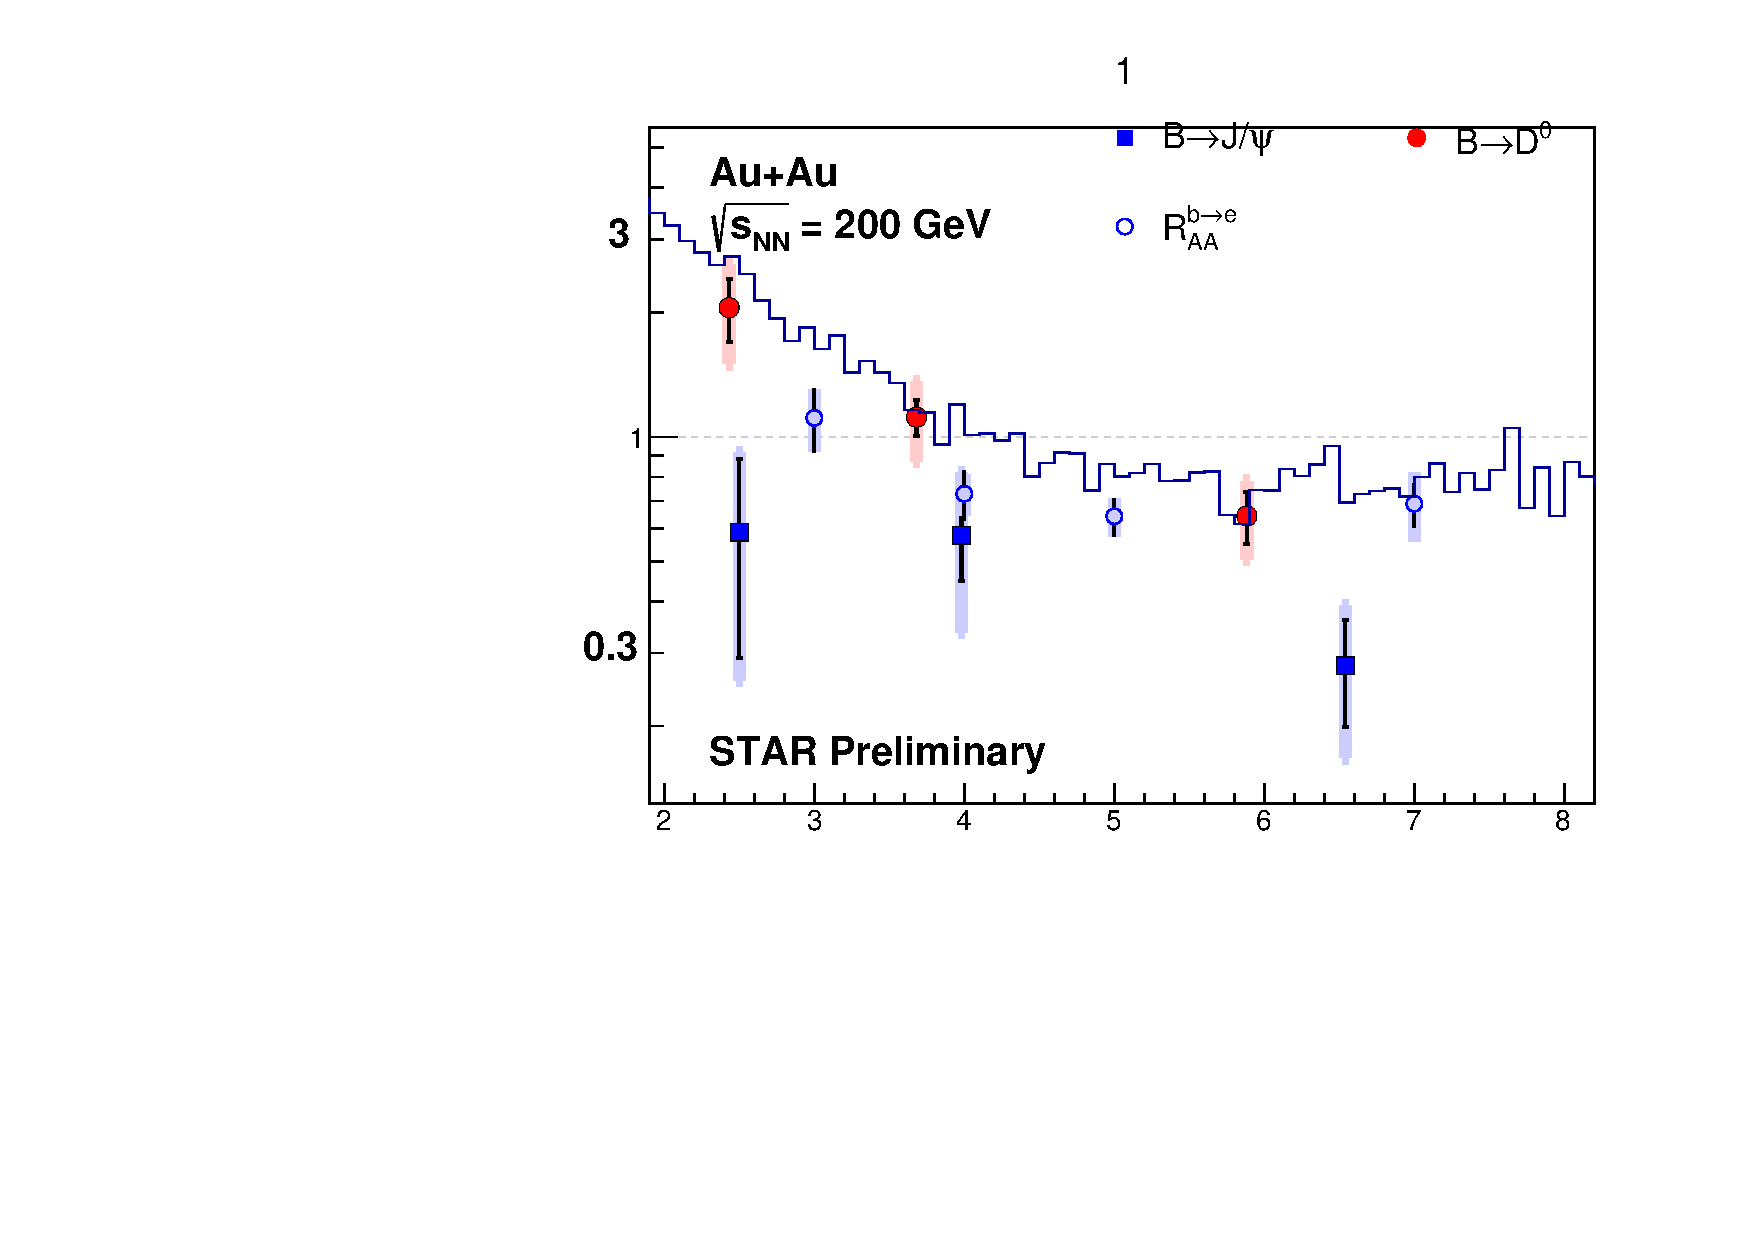
\includegraphics[width=8cm]{src/B2e.pdf}
	\caption{B2e $R_{AA}$}
\end{figure}
\end{frame}

\begin{frame}
\frametitle{结果}
\begin{figure}[h]
	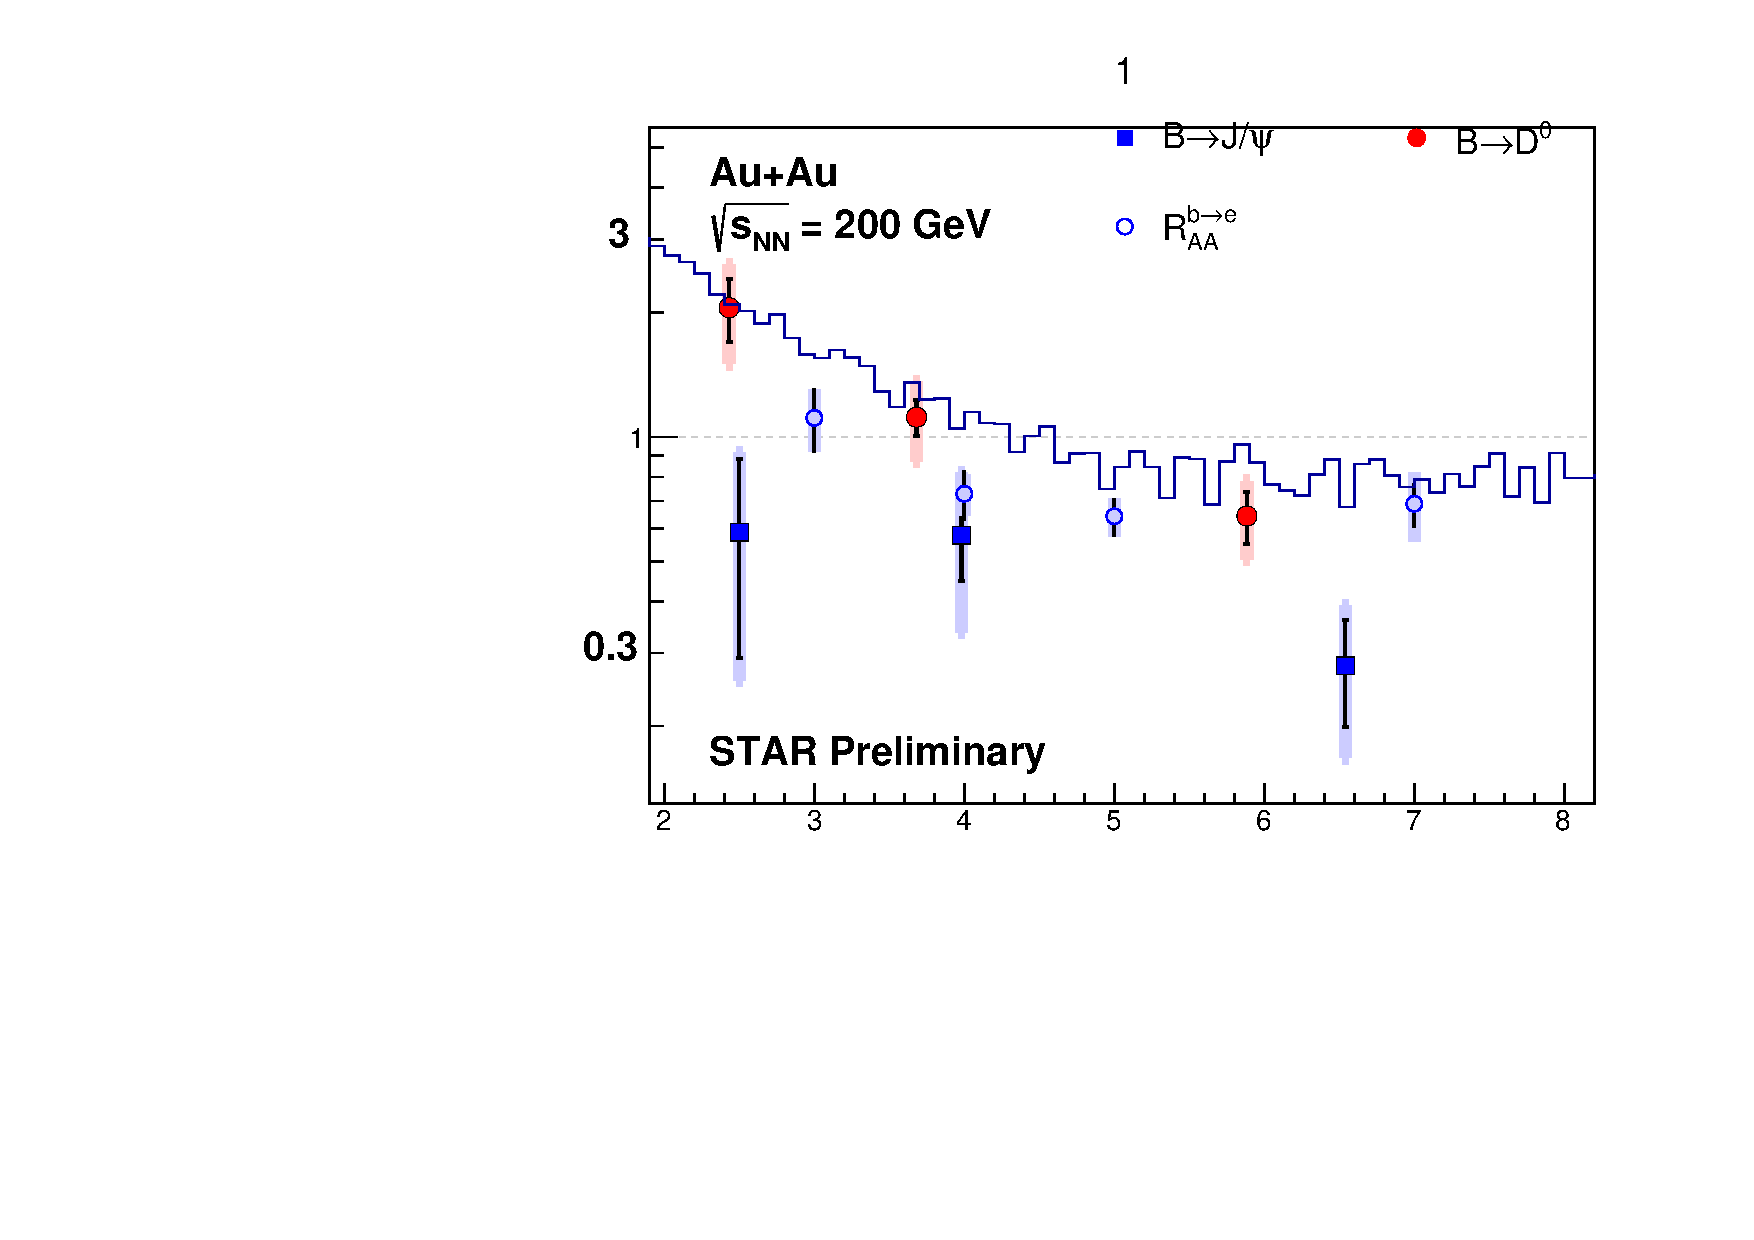
\includegraphics[width=8cm]{src/B2D0.pdf}
	\caption{B2D0 $R_{AA}$}
\end{figure}
\end{frame}
\begin{frame}
\frametitle{结果}
\begin{figure}[h]
	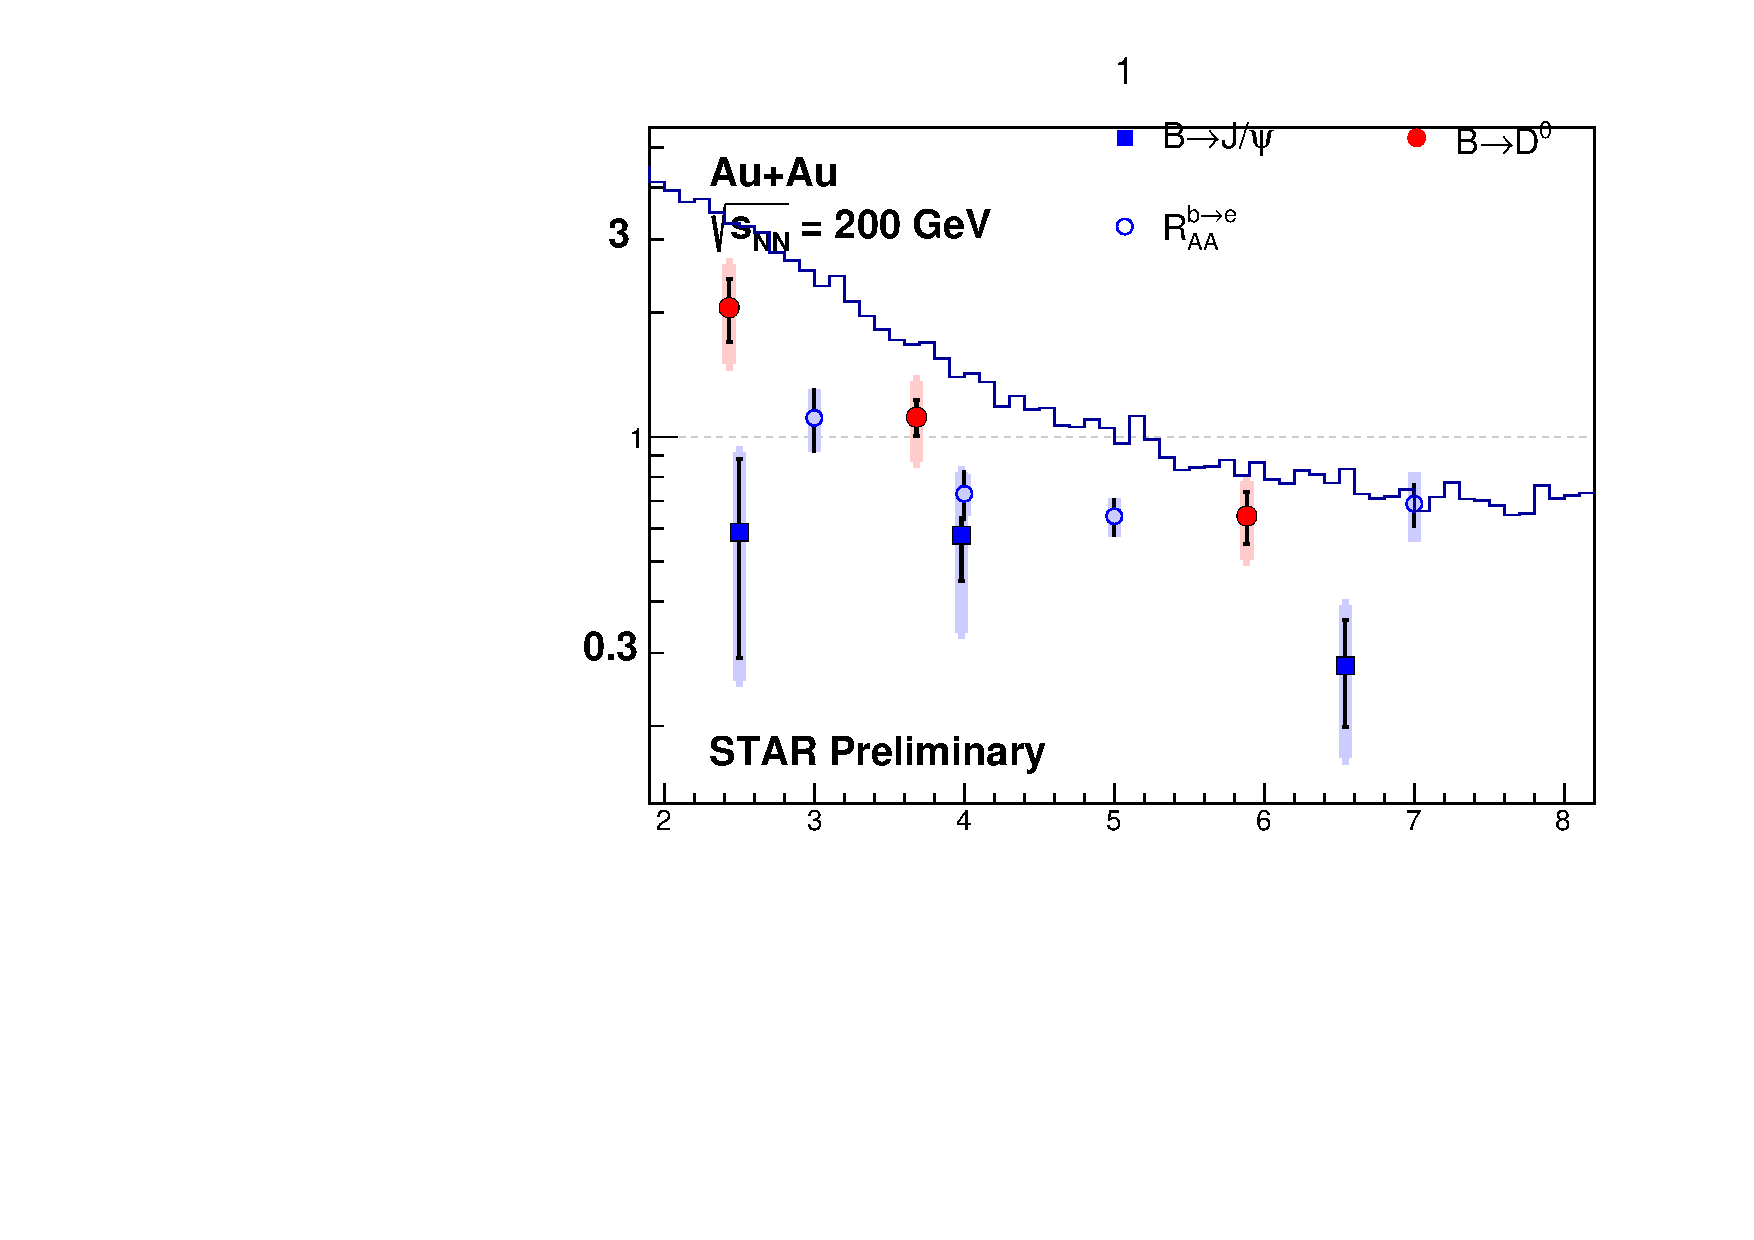
\includegraphics[width=8cm]{src/B2Jpsi.pdf}
	\caption{B2Jpsi $R_{AA}$}
\end{figure}
\end{frame}
\begin{frame}
	\frametitle{检查}
	\begin{figure}[h]
	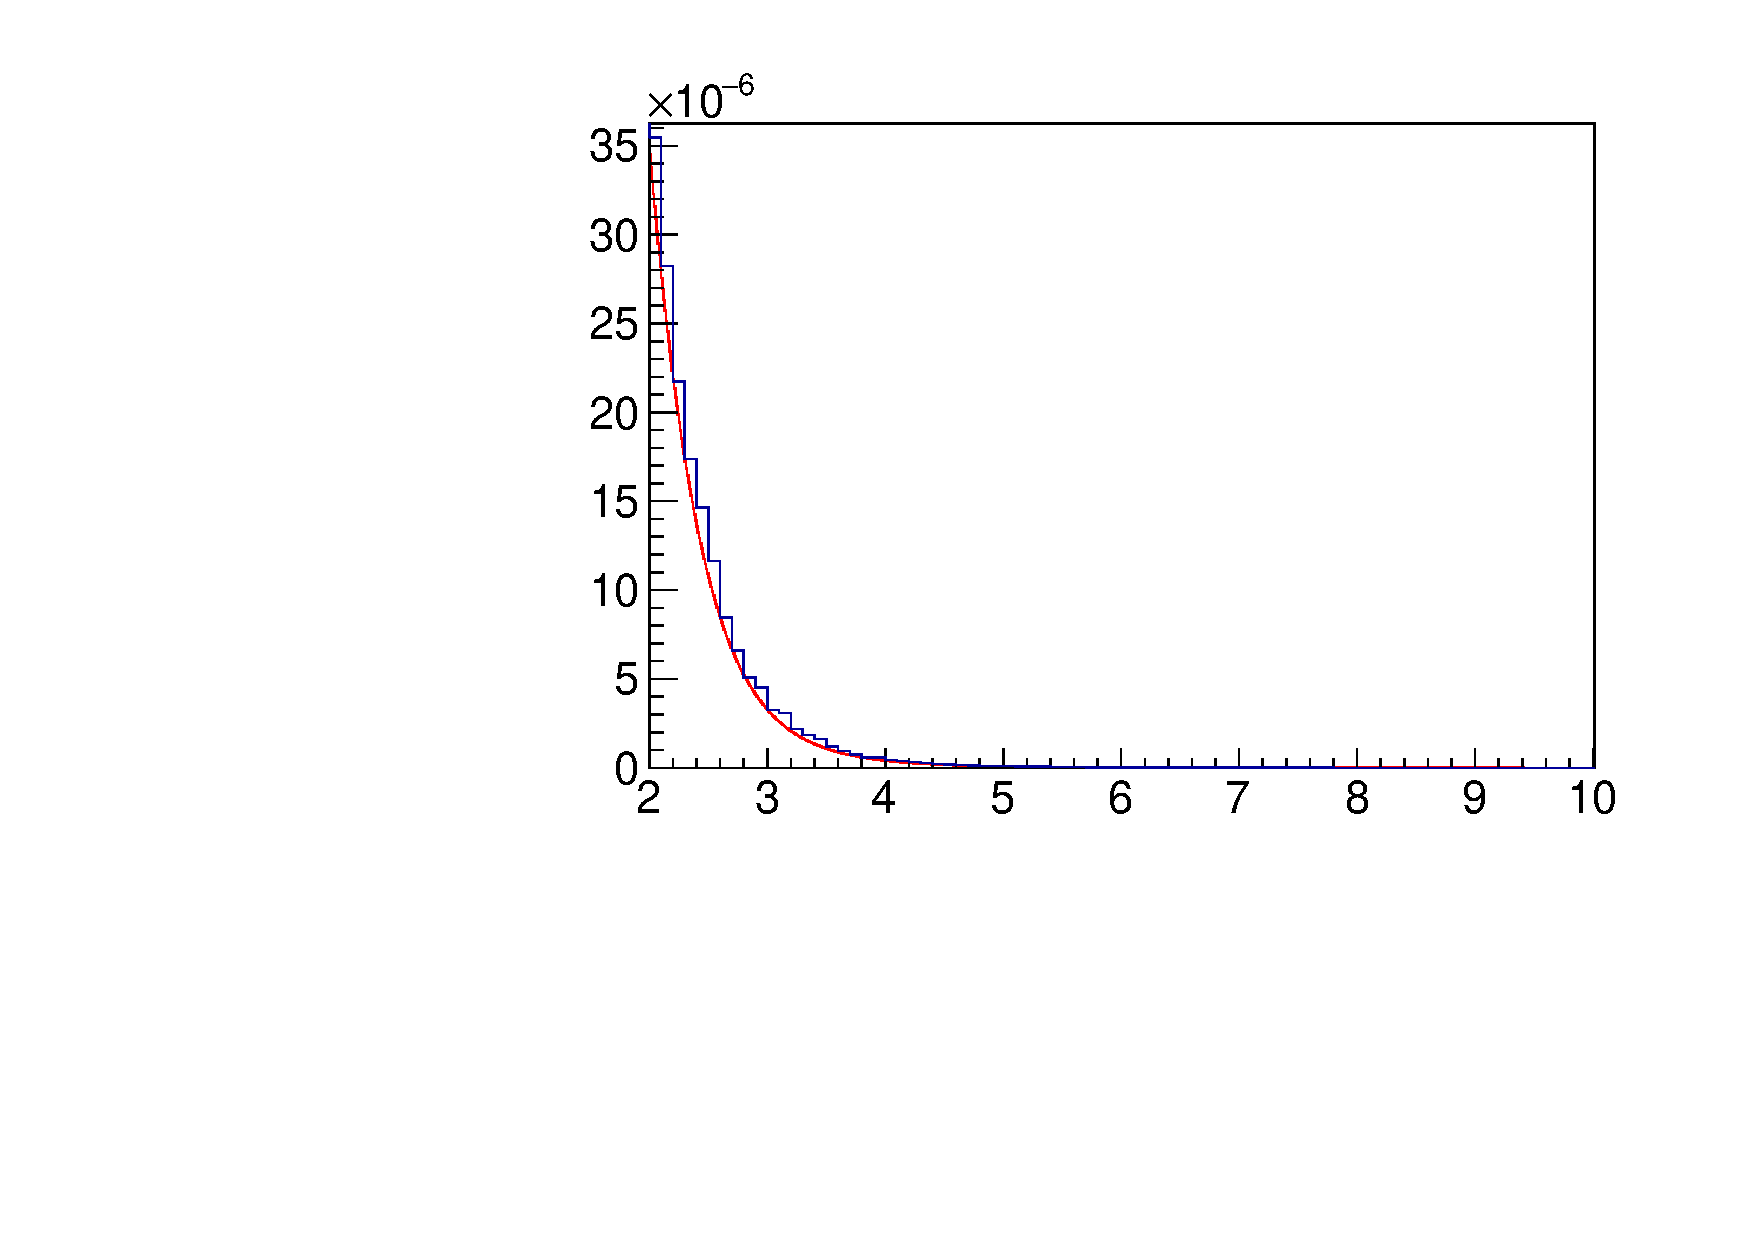
\includegraphics[width=8cm]{src/checke.pdf}
	\caption{B2echeck}
\end{figure}
\end{frame}

\begin{frame}
\frametitle{检查}
\begin{figure}[h]
	\includegraphics[width=8cm]{src/B2efonll.pdf}
	\caption{B2e $R_{AA}$, 对FONLL的检查}
\end{figure}
\end{frame}

\begin{frame}
	\frametitle{检查}
	\begin{figure}[h]
	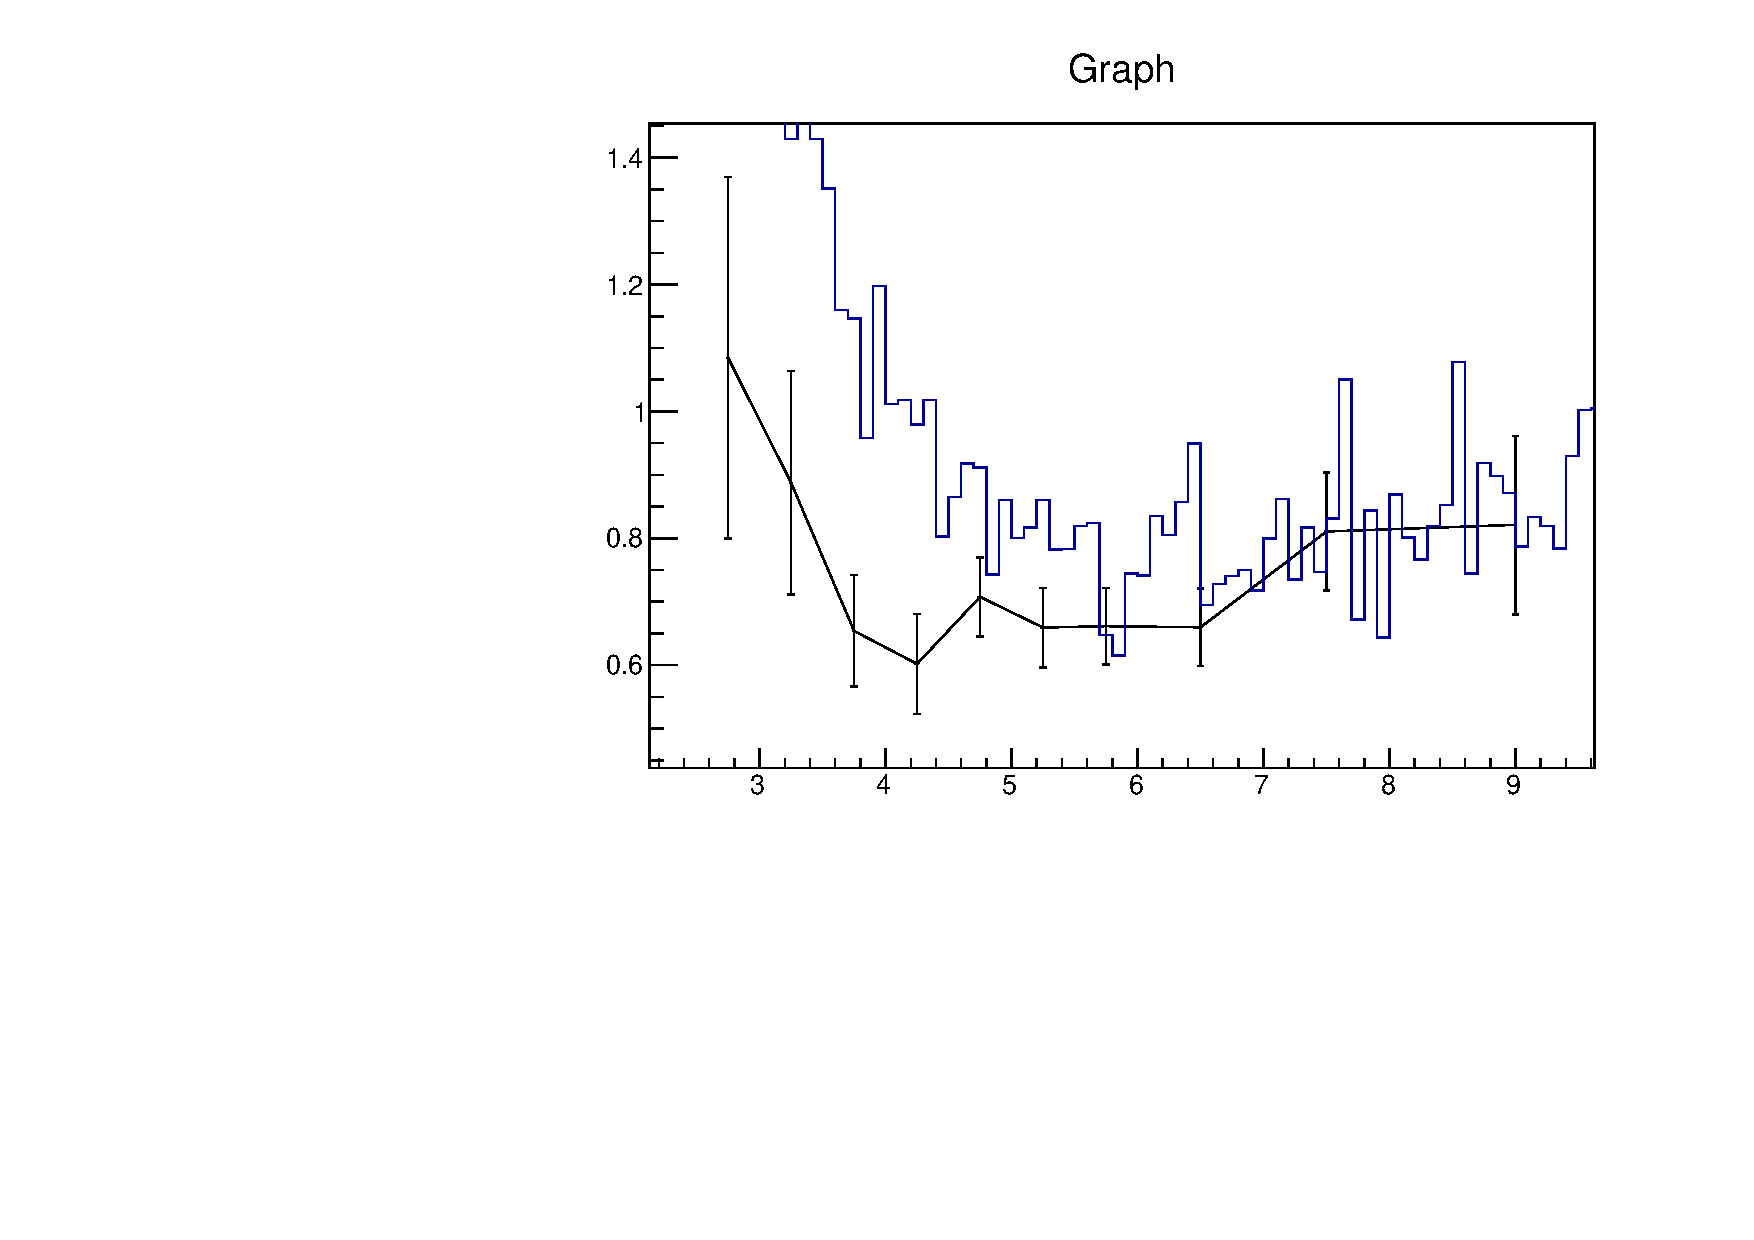
\includegraphics[width=8cm]{src/checkRaa.pdf}
	\caption{B2eRaacheck}
\end{figure}
\end{frame}

\begin{frame}
	\frametitle{检查}
	{\kaishu 数据: yield. 绘图时除以了$2\pi p_T\rd p_T\rd y$. $\rd y=2,\rd p_T = 1,2,3$. {\color{blue} 乘上$BR$}. 直方图除以了$N_{AA}=297$. 忽略了yield换算到截面乘以42mb的问题.}
	\begin{figure}[h]
	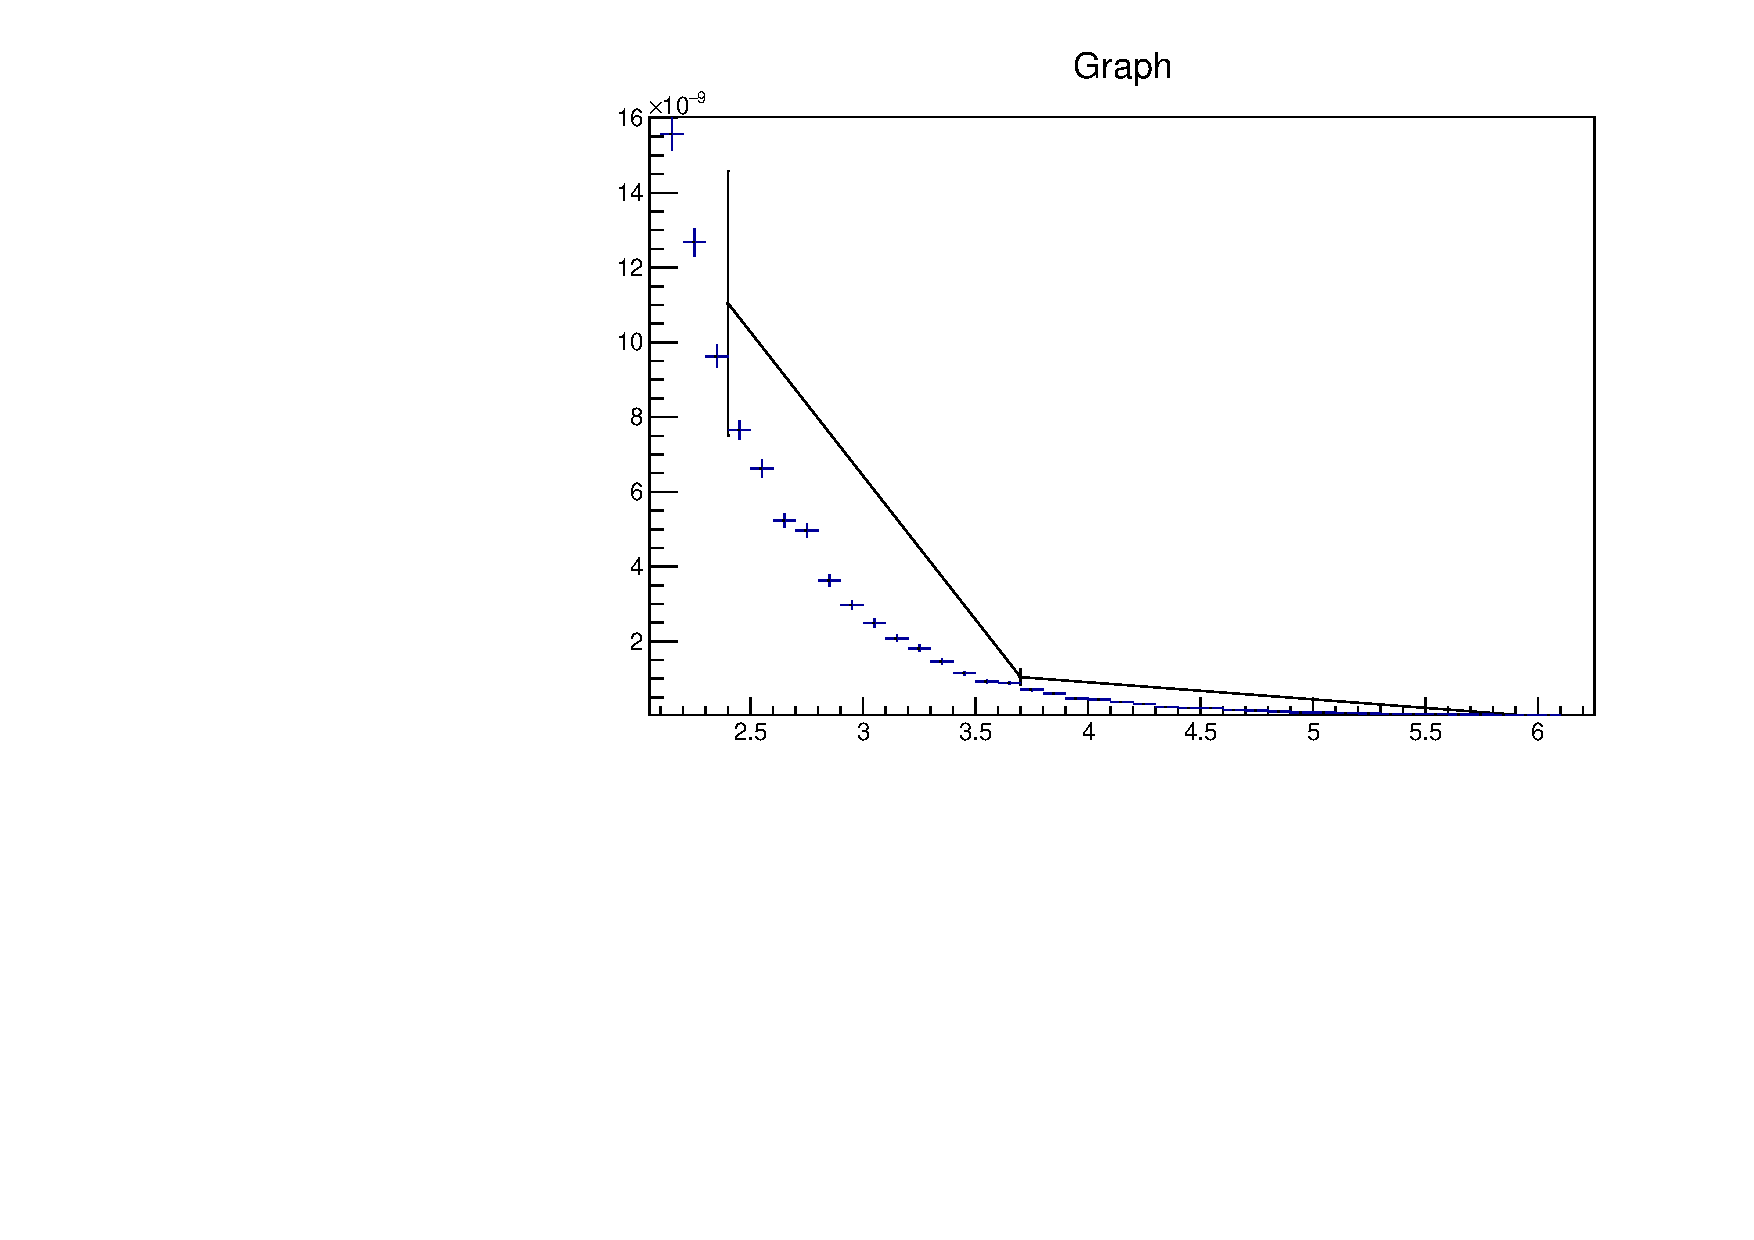
\includegraphics[width=6cm]{src/checkD0.pdf}
	\caption{B2D0check}
\end{figure}
\end{frame}

% \begin{frame}
% 	\frametitle{检查}
% 	\begin{figure}[h]
% 	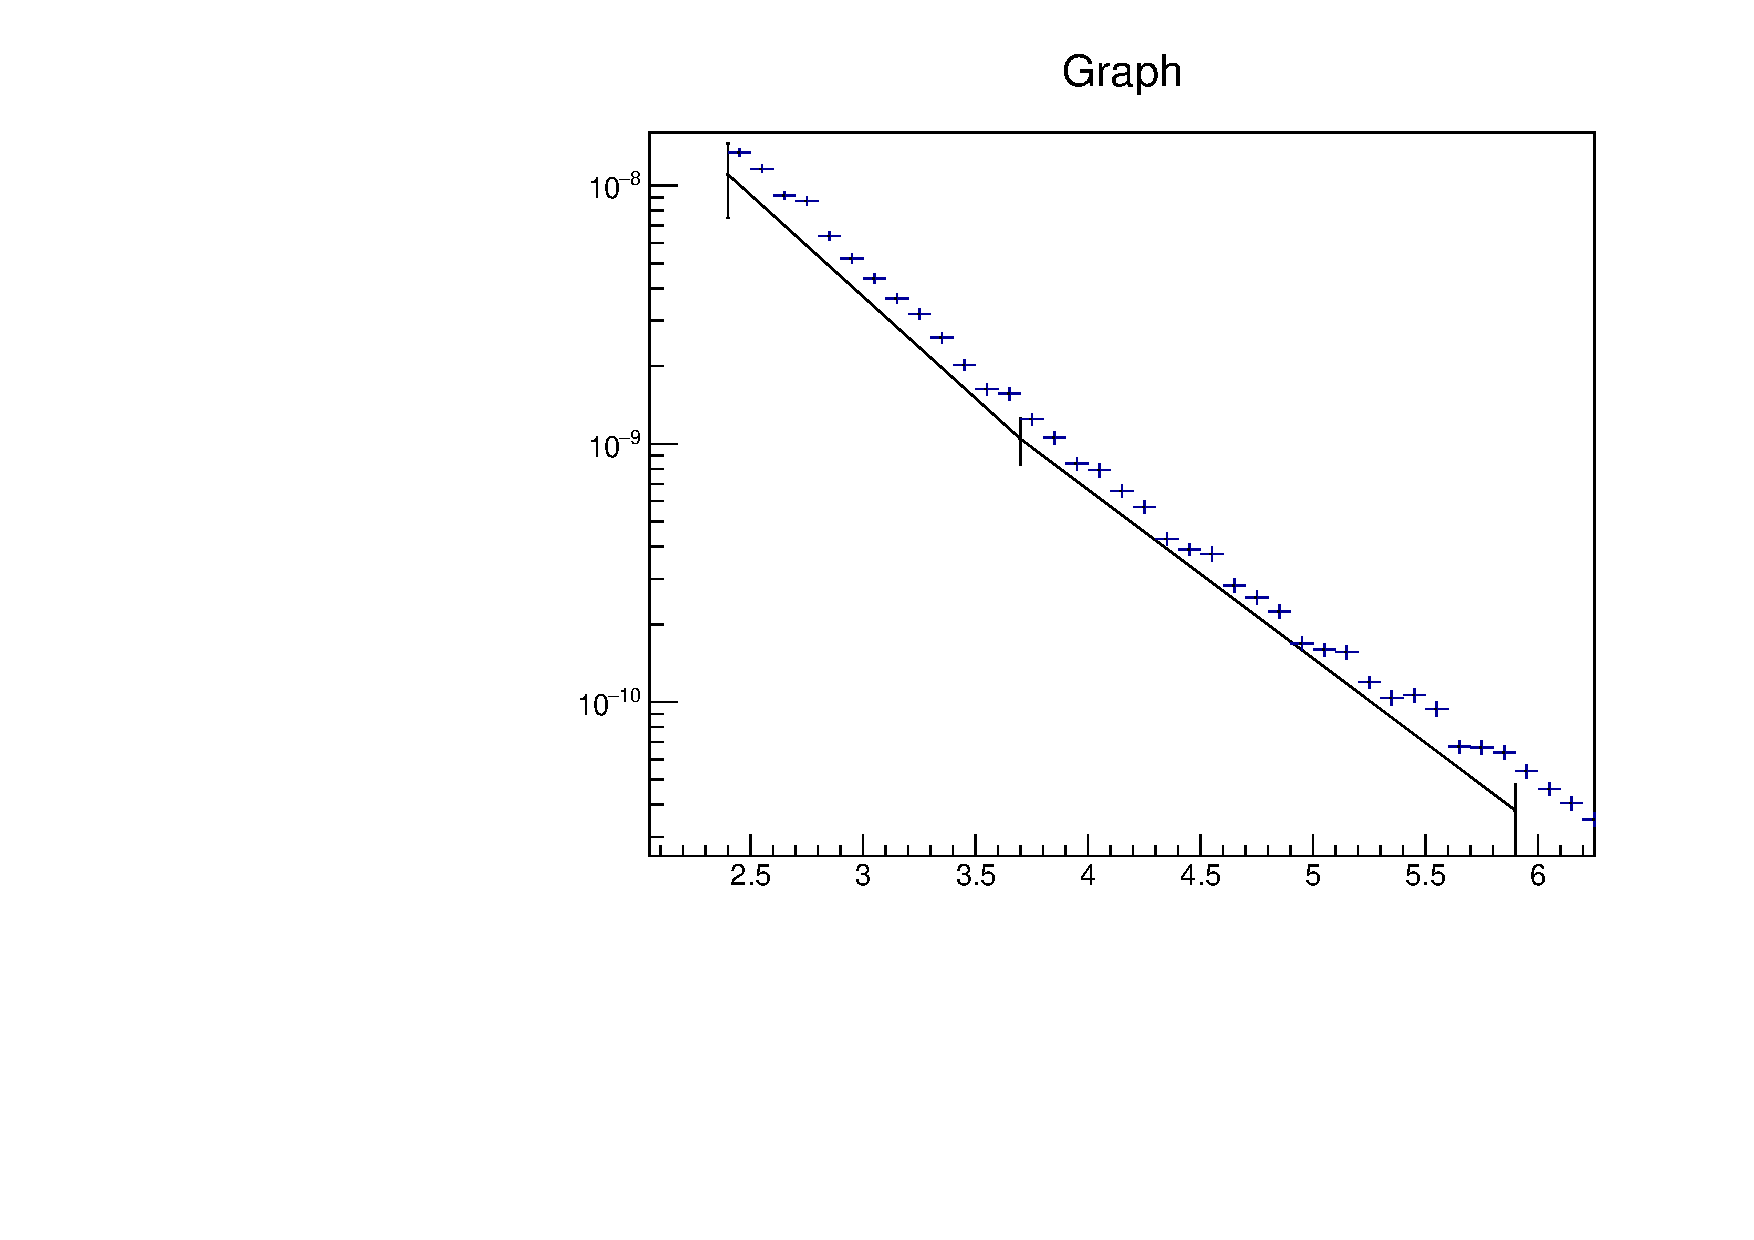
\includegraphics[width=8cm]{src/checkD0log.pdf}
% 	\caption{B2D0check}
% \end{figure}

% \end{frame}

\end{document}